\documentclass[10pt]{mypackage}

% sans serif font:
%\usepackage{cmbright}
%\usepackage{sfmath}
%\usepackage{bbold} %better blackboard bold

%serif font + different blackboard bold for serif font
\usepackage{newpxtext,eulerpx}
\renewcommand*{\mathbb}[1]{\varmathbb{#1}}
\renewcommand*{\hbar}{\hslash}

\pagestyle{fancy} %better headers
\fancyhf{}
\rhead{Avinash Iyer}
\lhead{Physics 310: Assignment 4}

\setcounter{secnumdepth}{0}

\begin{document}
\RaggedRight
\section{Chapter 11 Problems}%
\subsection{Problem 1}%
\begin{enumerate}[(a)]
  \item $\mathbf{F}\left(\mathbf{x}\right) = \frac{1}{\rho}\hat{\rho}$.
    \begin{center}
      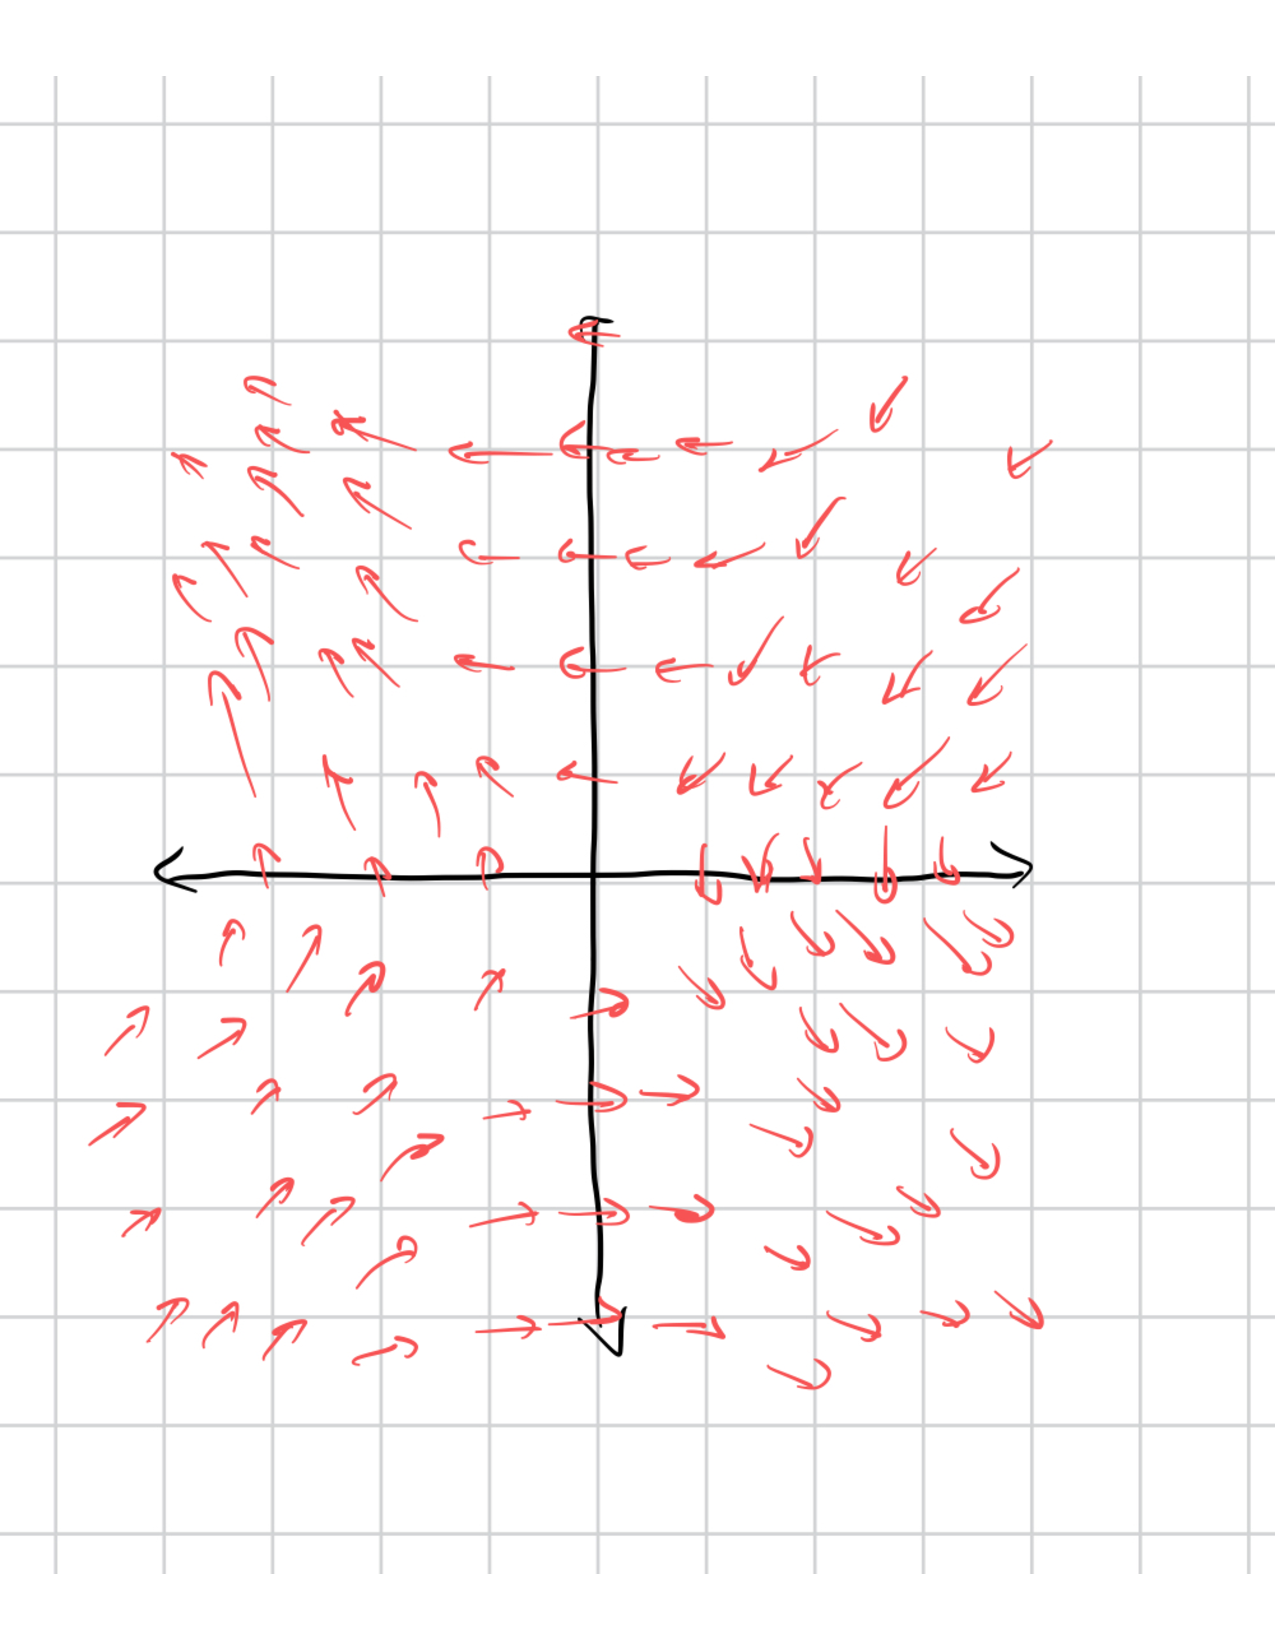
\includegraphics[width=10cm]{images/p_2a_1_11-1a.pdf}
    \end{center}
  \item $\mathbf{F}\left(\mathbf{x}\right) = y\hat{i} + x\hat{j}$.
    \begin{center}
      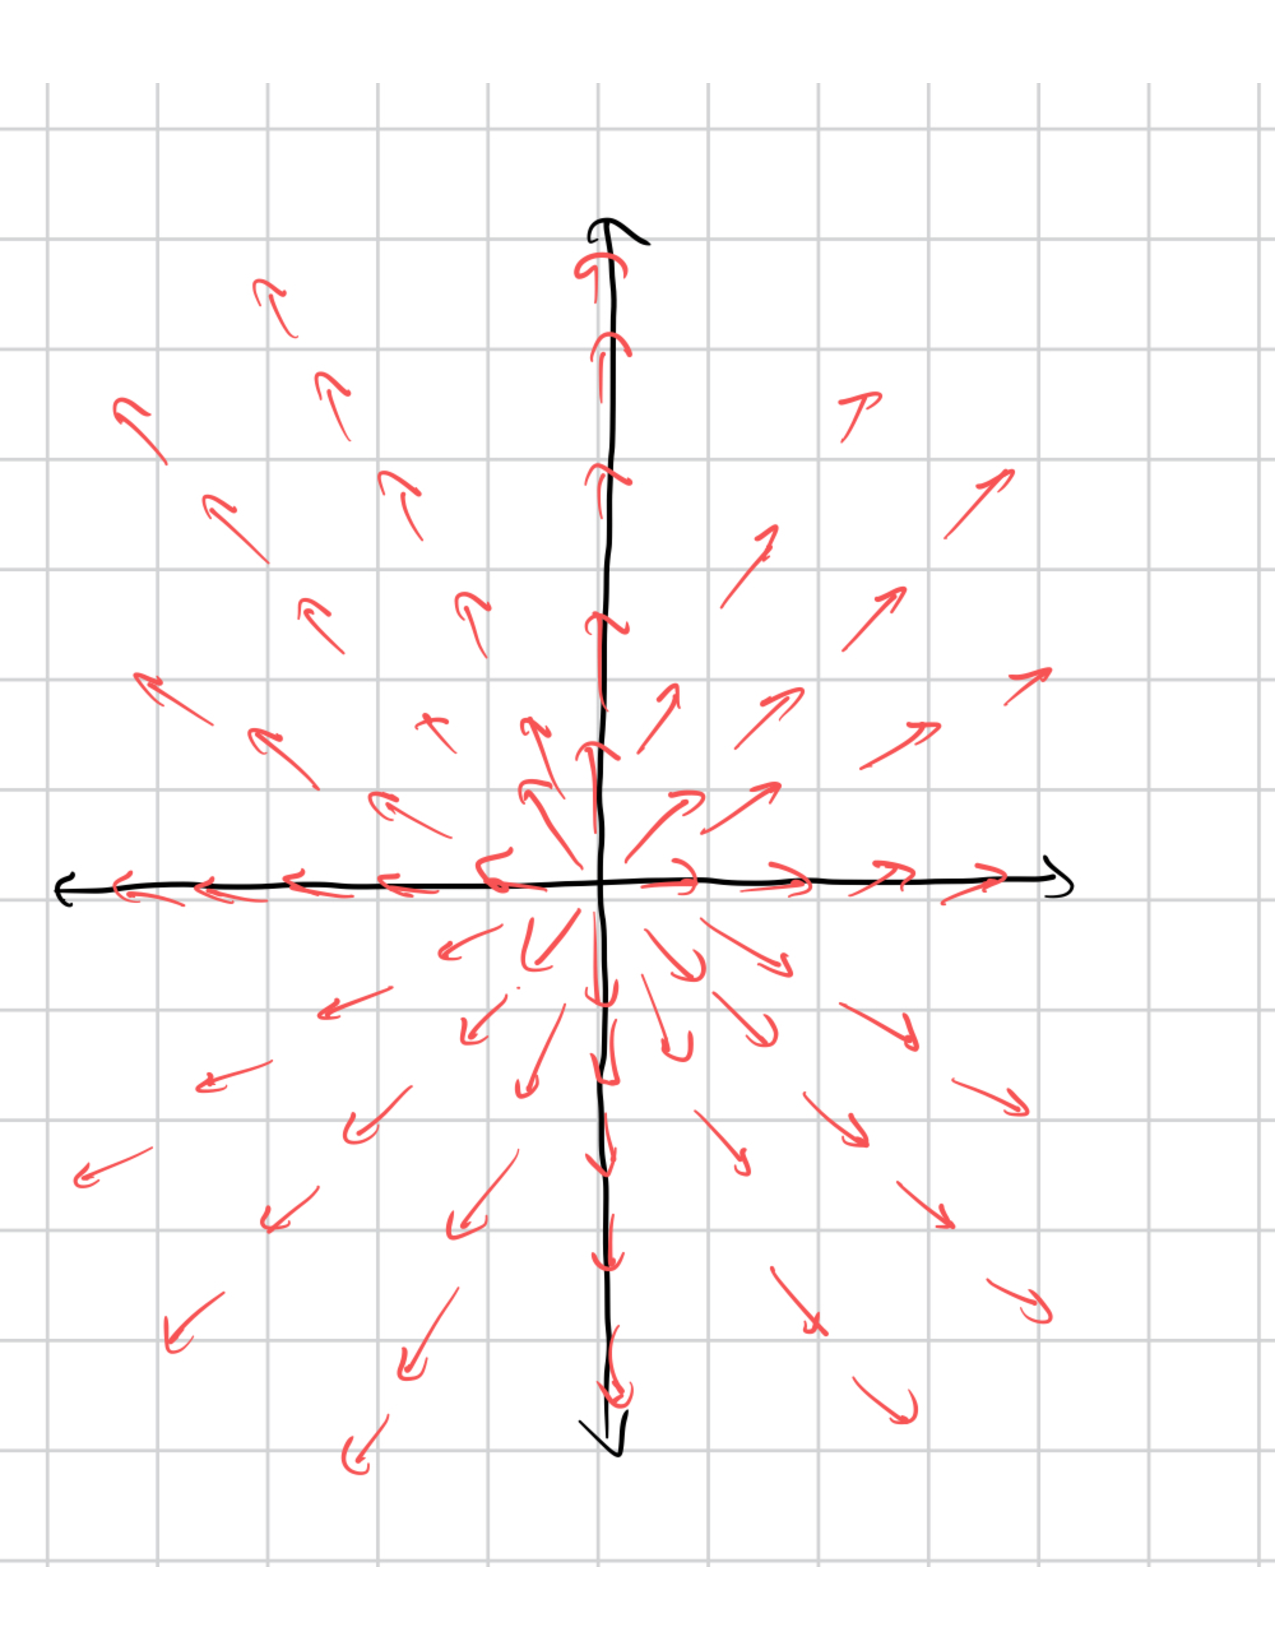
\includegraphics[width=10cm]{images/p_2a_1_11-1b.pdf}
    \end{center}
\end{enumerate}
\subsection{Problem 2}%
The parametrized streamlines for $\mathbf{v} = \left(-y,x\right)$ are of the form $r\cos t \hat{i} + r\sin t \hat{j}$.
\subsection{Problem 3}%
We can see that $\mathbf{E}$ and $\mathbf{B}$ are mutually perpendicular by taking the standard inner product
\begin{align*}
  \iprod{xy^2\hat{i} + x^2y\hat{j}}{x^2y\hat{i} - xy^2\hat{j}} &=0.
\end{align*}
Additionally, for $\mathbf{E}$,
\begin{align*}
  \diff{y}{t} &= x^2 y\\
  \diff{x}{t} &= xy^2\\
  \diff{y}{x} &= \frac{x}{y}\\
  y^2 &= x^2 + K,
\end{align*}
and for $\mathbf{B}$,
\begin{align*}
  \diff{y}{t} &= -xy^2\\
  \diff{x}{t} &= x^2 y\\
  \diff{y}{x} &= -\frac{y}{x}\\
  y &= \frac{K}{x}.
\end{align*}
\subsection{Problem 4}%
\begin{enumerate}[(a)]
  \item 
    \begin{align*}
      \int_{V}^{} \mathbf{E}\left(\mathbf{r}\right)\:d^3x &= \int_{0}^{\pi/2}\int_{0}^{2\pi}\int_{0}^{R} \hat{r}\sin\theta \:drd\phi d\theta\\
      \int_{V}^{} \mathbf{E}\left(\mathbf{r}\right)\:d^3 x &= \int_{-R}^{R}\int_{-\sqrt{R^2-x^2}}^{\sqrt{R^2-x^2}}\int_{0}^{\sqrt{R^2-x^2 - y^2}} \frac{x\hat{i} + y\hat{j} + z\hat{k}}{\left(x^2 + y^2 + z^2\right)^{3/2}}\:dz dy dx
    \end{align*}
  \item 
    \begin{align*}
      \int_{V}^{} \mathbf{E}\left(\mathbf{r}\right)\:d^3 x &= \int_{0}^{\pi/2}\int_{0}^{2\pi}\int_{0}^{R} \sin\theta \left(\cos\phi\sin\theta\hat{i} + \sin\phi\sin\theta\hat{j} + \cos\theta\hat{k}\right)\:dr d\phi d\theta
    \end{align*}
    This integral is more practical than the pure forms since the basis is position-independent and the integral is not a giant mess.
  \item Using symmetry, since $\cos\phi$ is integrated from $0$ to $2\pi$ and $\sin\phi$ is integrated from $0$ to $2\pi$, both the $\hat{i}$ and $\hat{j}$ components are $0$.
    \begin{align*}
      \int_{0}^{\pi/2} \sin^2\theta \int_{0}^{2\pi}\cos\phi\int_{0}^{R}\:dr d\phi d\phi &= 0\\
      \int_{0}^{\pi/2} \sin^2\theta \int_{0}^{2\pi}\sin\phi\int_{0}^{R}\:dr d\phi d\phi &= 0
    \end{align*}
  \item Evaluating the $\hat{k}$ component,
    \begin{align*}
      \int_{0}^{\pi/2}\sin\theta\cos\theta \int_{0}^{2\pi}\int_{0}^{R} \:dr d\phi d\theta &= 2\pi R \int_{0}^{\pi/2} \sin\theta\cos\theta\:d\theta\\
                                                                                          &= \pi R.
    \end{align*}
\end{enumerate}
\subsection{Problem 5}%
\begin{align*}
  \mathbf{R}_{\text{cm}} &= \frac{1}{M}\int_{S}^{} \mathbf{r}\:dm\\
                         &= \frac{\sigma}{M}\int_{-\ell/2}^{\ell/2}\int_{0}^{\pi} \left(R\cos\phi\hat{i} + R\sin\phi\hat{j} + z\hat{k} \right)R\:d\phi dz\\
                         &= \frac{\sigma}{M} \left(2R^2\right) \hat{j}.
\end{align*}
\section{Chapter 12 Problems}%
\subsection{Problem 1}%
\begin{enumerate}[(a)]
  \item Letting $f\left(\mathbf{x}\right) = \rho$, we have
    \begin{align*}
      \nabla f &= \hat{\rho}
    \end{align*}
    in cylindrical coordinates, and
    \begin{align*}
      \nabla f &= \frac{x}{\sqrt{x^2 + y^2}}\hat{i} + \frac{y}{\sqrt{x^2 + y^2}}\hat{j}
    \end{align*}
    in Cartesian coordinates. These results are equal to each other by the definition of $\hat{\rho}$.
  \item Letting $f\left(\mathbf{x}\right)= y$, we have
    \begin{align*}
      \nabla f &= \hat{j}
    \end{align*}
    in Cartesian coordinates, and
    \begin{align*}
      \nabla f &= \sin\phi\hat{\rho} + \cos\phi\hat{\phi},
    \end{align*}
    which yields $\hat{j}$ under the coordinate conversion.
  \item Letting $f\left(\mathbf{x}\right) = z\rho^2$, we have
    \begin{align*}
      \nabla f &= 2\rho z \hat{\rho} + \rho^2\hat{k}
    \end{align*}
    in cylindrical coordinates, and
    \begin{align*}
      \nabla f &= 2xz\hat{i} + 2yz\hat{j} + \left(x^2 + y^2\right)\hat{k},
    \end{align*}
    which is equal under the coordinate conversion.
  \item Letting $f\left(\mathbf{x}\right) = \rho^2\tan\phi$, we have
    \begin{align*}
      \nabla f &= 2\rho\tan\phi\hat{\rho} + \rho\sec^2\phi\hat{\phi}
    \end{align*}
    and
    \begin{align*}
      \nabla f &= \left(y - \frac{y^3}{x^2}\right)\hat{i} + \left(x + \frac{3y^2}{x}\right)\hat{j},
    \end{align*}
    which is equal under the coordinate conversion.
\end{enumerate}
\subsection{Problem 2}%
\begin{enumerate}[(a)]
  \item Let $f\left(\mathbf{x}\right) = r\sin\theta\cos\phi$. Then,
    \begin{align*}
      \nabla f &= \pd{f}{r}\hat{r} + \frac{1}{r\sin\theta}\pd{f}{\phi}\hat{\phi} + \frac{1}{r}\pd{f}{\theta}\hat{\theta}\\
               &= \sin\theta\cos\phi\hat{r} - \sin\phi\hat{\phi} + \cos\theta\cos\phi\hat{\theta},
    \end{align*}
    and
    \begin{align*}
      \nabla \cdot \left(\nabla f\right) &= 0.
    \end{align*}
  \item Let $f\left(\mathbf{x}\right) = \ln \rho^2$. Then,
    \begin{align*}
      \nabla f &= \frac{2}{\rho}\hat{\rho}\\
      \nabla \cdot \left(\nabla f\right) &= -\frac{2}{\rho^2}.
    \end{align*}
  \item Let $f\left(\mathbf{x}\right) = x\cos y$. Then,
    \begin{align*}
      \nabla f &= \cos y \hat{i} - x\sin y \hat{j},
    \end{align*}
    and
    \begin{align*}
      \nabla \cdot \left(\nabla f\right) &= -x\cos y
    \end{align*}
  \item Let $f\left(\mathbf{x}\right) = x\left(y^2 - 1\right)$. Then,
    \begin{align*}
      \nabla f &= \left(y^2 - 1\right)\hat{i} + 2xy\hat{j},
    \end{align*}
    and
    \begin{align*}
      \nabla \cdot \left(\nabla f\right) &= 2x.
    \end{align*}
\end{enumerate}
\subsection{Problem 3}%
\begin{enumerate}[(a)]
  \item 
    \begin{align*}
      \mathbf{r} &= \vec{r}\\
                 &= r\hat{r}\\
      \nabla \cdot \left(r\hat{r}\right) &= 1\\
      \nabla \times \left(r\hat{r}\right) &= 0
    \end{align*}
  \item 
    \begin{align*}
      \mathbf{r} &= \frac{\hat{r}}{r}\\
      \nabla \cdot \left(\frac{\hat{r}}{r}\right) &= -\frac{1}{r^2}\\
      \nabla \times \left(\frac{\hat{r}}{r}\right) &= 0.
    \end{align*}
  \item 
    \begin{align*}
      \mathbf{r} &= \frac{1}{r^2}\hat{\theta}\\
      \nabla \cdot \left(\frac{1}{r^2}\hat{\theta}\right) &= 0\\
      \nabla \times \left(\frac{1}{r^2}\hat{\theta}\right) &= \frac{1}{r}\left(\pd{}{r}\left(\frac{1}{r}\right)\right)\hat{\phi}\\
                                                           &= -\frac{1}{r^3}\hat{\phi}.
    \end{align*}
  \item 
    \begin{align*}
      \mathbf{r} &= \rho z \hat{\phi}\\
      \nabla \cdot \left(\rho z \hat{\phi}\right) &= 0\\
      \nabla \times \left(\rho z \hat{\phi}\right) &= -\rho \hat{\rho} + 2\rho z \hat{z}.
    \end{align*}
\end{enumerate}
\subsection{Problem 6}%
\begin{align*}
  \mathbf{B} &= \frac{1}{x^2 + y^2}\left(-y\hat{i} + x\hat{j}\right)\\
             &= \frac{1}{\rho}\hat{\phi}\\
  \nabla \times \mathbf{B} &= \left(\frac{\partial}{\partial x}\left(\frac{x}{x^2 + y^2}\right) - \frac{\partial}{\partial y}\left(\frac{-y}{x^2 + y^2}\right)\right)\hat{k}\\
                           &= \left(\frac{2}{x^2 + y^2} - \frac{2x^2}{\left(x^2 + y^2\right)^2} - \frac{2y^2}{\left(x^2 + y^2\right)^2}\right)\\
                           &= 0\\
  \nabla \times \mathbf{B} &= 0.
\end{align*}
\subsection{Problem 7}%
\begin{align*}
  \nabla \cdot \left(\nabla f(r)\right) &= \nabla \cdot \left(\pd{f}{r}\right)\hat{r}\\
                                        &= \frac{1}{r^2}\pd{}{r}\left(r^2\left(\pd{f}{r}\right)\right)\\
                                        &= \frac{1}{r^2}\pd{}{r}\left(r^2\pd{f}{r}\right).
\end{align*}
\subsection{Problem 9}%
\begin{align*}
  \nabla\cdot \left(\nabla\left(fg\right)\right) &= \nabla \cdot \left(g\nabla f + f\nabla g\right)\\
                                                 &= \nabla \cdot \left(g\nabla f\right) + \nabla \cdot \left(f\nabla g\right)\\
                                                 &= \nabla g\cdot\nabla f + g\left(\nabla \cdot \nabla f\right) + \nabla f \cdot \nabla g + f\left(\nabla \cdot \nabla g\right).
\end{align*}
This expression is equal to $g\nabla^2 f + f\nabla^2 g$ if and only if $\nabla f \cdot \nabla g = 0$ on the domain of $f$ and $g$ (i.e., that $\nabla f$ and $\nabla g$ are orthogonal to each other).
\subsection{Problem 15}%

\begin{enumerate}[(a)]
  \item 
    \begin{center}
      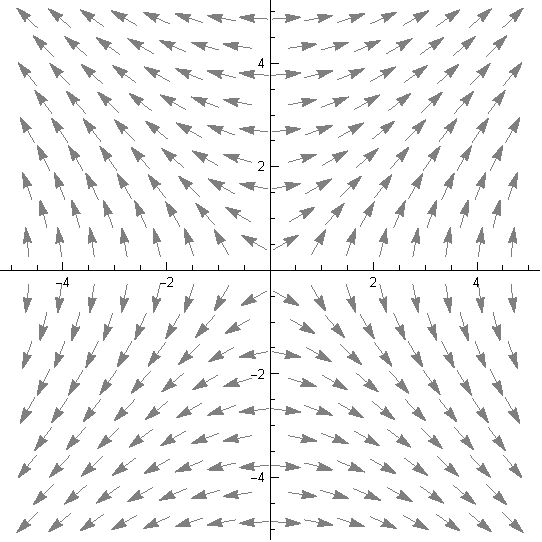
\includegraphics[width=10cm]{images/p_2a_1_12-19a.pdf}
    \end{center}
    Upon inspection, this field appears to have a significant amount of ``surge,'' but not any ``swirl,'' implying that its curl should be zero and its divergence positive.
    \begin{align*}
      \nabla \cdot \mathbf{E} &= y^2 + x^2\\
      \nabla \times \mathbf{E} &= \left(\pd{}{x}\left(x^2 y\right) - \pd{}{y}\left(xy^2\right)\right)\hat{k}\\
                               &= 0.
    \end{align*}
  \item 
    \begin{center}
      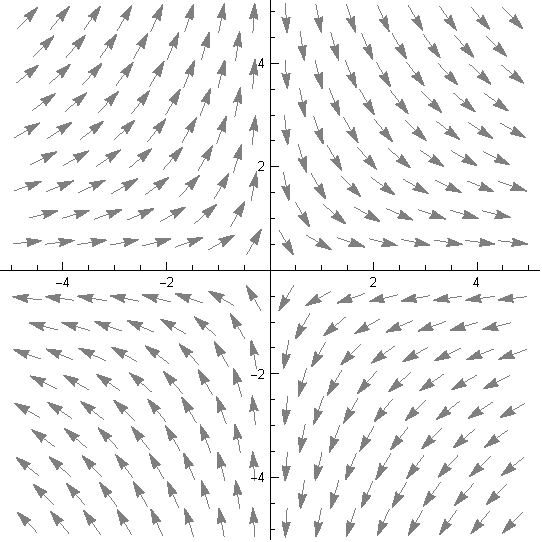
\includegraphics[width=10cm]{images/p_2a_1_12-19b.pdf}
    \end{center}
    Upon inspection, this field appears to have a significant amount of ``swirl,'' but not any ``surge,'' implying that its divergence should be zero and its curl should be nonzero.
    \begin{align*}
      \nabla \cdot \mathbf{B} &= \pd{}{x}\left(x^2 y\right) - \pd{}{y}\left(xy^2\right)\\
                              &= 0\\
      \nabla \times \mathbf{B} &= \left(\pd{}{x}\left(-xy^2\right) - \pd{}{y}\left(x^2y\right)\right)\hat{k}\\
                               &= -\left(x^2 + y^2\right)\hat{k}.
    \end{align*}
\end{enumerate}
\subsection{Problem 19}%
\begin{enumerate}[(a)]
  \item 
    \begin{align*}
      \nabla \cdot \left(\phi \mathbf{A}\right) &= \sum_{i,j}\pd{}{i}\left(\phi A_{j}\right)\delta_{ij}\\
                                                &= \sum_{i}\pd{}{i}\left(\phi A_i\right)\\
                                                &= \sum_{i}\left(A_i\pd{}{i}\phi + \phi \pd{}{i}A_i\right)\\
                                                &= \mathbf{A}\cdot \left(\nabla \phi\right) + \phi \left(\nabla \cdot \mathbf{A}\right).
    \end{align*}
  \item 
    \begin{align*}
      \nabla \times \left(\phi \mathbf{A}\right) &= 
    \end{align*}
\end{enumerate}
\section{Chapter 13 Problems}%
\subsection{Problem 2}%

\end{document}
